\documentclass[conference]{IEEEtran}
\usepackage{times}

% numbers option provides compact numerical references in the text. 
\usepackage[numbers]{natbib}
\usepackage{multicol}
\usepackage[bookmarks=true]{hyperref}

\pdfinfo{
   /Author (Homer Simpson)
   /Title  (Robots: Our new overlords)
   /CreationDate (D:20101201120000)
   /Subject (Robots)
   /Keywords (Robots;Overlords)
}

\begin{document}

% paper title
\title{Template paper for the \\Robotics: Science and Systems Conference}

% You will get a Paper-ID when submitting a pdf file to the conference system
\author{Author Names Omitted for Anonymous Review. Paper-ID [add your ID here]}

%\author{\authorblockN{Michael Shell}
%\authorblockA{School of Electrical and\\Computer Engineering\\
%Georgia Institute of Technology\\
%Atlanta, Georgia 30332--0250\\
%Email: mshell@ece.gatech.edu}
%\and
%\authorblockN{Homer Simpson}
%\authorblockA{Twentieth Century Fox\\
%Springfield, USA\\
%Email: homer@thesimpsons.com}
%\and
%\authorblockN{James Kirk\\ and Montgomery Scott}
%\authorblockA{Starfleet Academy\\
%San Francisco, California 96678-2391\\
%Telephone: (800) 555--1212\\
%Fax: (888) 555--1212}}


% avoiding spaces at the end of the author lines is not a problem with
% conference papers because we don't use \thanks or \IEEEmembership


% for over three affiliations, or if they all won't fit within the width
% of the page, use this alternative format:
% 
%\author{\authorblockN{Michael Shell\authorrefmark{1},
%Homer Simpson\authorrefmark{2},
%James Kirk\authorrefmark{3}, 
%Montgomery Scott\authorrefmark{3} and
%Eldon Tyrell\authorrefmark{4}}
%\authorblockA{\authorrefmark{1}School of Electrical and Computer Engineering\\
%Georgia Institute of Technology,
%Atlanta, Georgia 30332--0250\\ Email: mshell@ece.gatech.edu}
%\authorblockA{\authorrefmark{2}Twentieth Century Fox, Springfield, USA\\
%Email: homer@thesimpsons.com}
%\authorblockA{\authorrefmark{3}Starfleet Academy, San Francisco, California 96678-2391\\
%Telephone: (800) 555--1212, Fax: (888) 555--1212}
%\authorblockA{\authorrefmark{4}Tyrell Inc., 123 Replicant Street, Los Angeles, California 90210--4321}}


\maketitle

\begin{abstract}
We consider the problem of learning to manipulate deformable objects
through learning from demonstrations.  Recent
work~\cite{Schulmanetal_IROS2013, Schulmanetal_ISRR2013} has shown
promising results in enabling robotic manipulation of deformable
objects through learning from demonstrations.  Their approach is able
to generalize from a single demonstration, and suggests a nearest
neighbor approach to decide which demonstration to generalize from for
a given test situation.  Such a nearest neighbor approach, however,
ignores important aspects of the problem:  brittleness (versus
robustness) of demonstrations when generalized through this process,
and the extent to which a demonstration makes progress towards the goal.

In this paper, we present a max-margin q-learning-based solution
to the demonstration selection problem that
can account for the variability in robustness of demonstrations and the
sequential nature of our tasks.   We also present experimental
validation of our approach.  We developed a knot-tying benchmark for
evaluating the effectiveness of
our proposed approach.   The
nearest neighbor approach described in \citet{Schulmanetal_ISRR2013} achieves a
68.8\% success rate. Our approach achieves a success rate of 95.2\%.
\end{abstract}


\IEEEpeerreviewmaketitle

\section{Introduction}
The recent commercial availablity of relatively cheap mobile robots such as Baxter and the UBR 1 
creates a very real possiblity for widespread appliation of robotics to mobile manipulation tasks.
There are huge economic gains to be had from the deployment of robotics in settings that range from homes to factories.
Our goal is to endow robots with the ability to execute complex, goal-directed, tasks in these unstructured settings.

These problems are characterized by state and action spaces that are high-dimensional and continuous.
The computational complexity faced by a robotic agent makes general solution of these problems difficult.
In modern factories, this is mitigated through intelligent design of environments and manipulation policies.
However, the design time and the skill required on the part of system designers prohibits application of these approaches for unstructured settings and more complex task.
Deformable object manipulation present an especially challenging scenario as modelling or tracking the underlying state of the world is a challenging task \cite{SchulmanLeeHoAbbeel_ICRA2013,Javdanietal_2011,Haehnel03a}.

One way to mitigate these issues is to frame our problem as one of learning from demonstrations.
Rather than starting from scratch in each scenario, we generalize from an expert demonstration.

A recent approach makes use of \emph{trajectory transfer} through the use of non-rigid registration to solve this problem.
When faced with a novel scenario, trajectory tranfers fits a function $f:\mathbb{R}^3 \rightarrow \mathbb{R}^3$ that warps a demonstration scene to a novel setting.
The demonstrated trajectory is then warped with this function and the result is executed. 
This has been shown to be effective for many complex task, including knot-tying and suturing \cite{Schulmanetal_ISRR2013, Schulmanetal_IROS2013}.\dhm{needs several citations}

There are limits to how well a single trajectory can transfer. 
Instead we provide a library of demonstrations and a method that selects which trajectory to transfer.
This enables our trajectory transfer systems to perform complex tasks by sequencing several trajecotry generalizations.
Selecting a demonstration that will generalize well to a particular scenario is integral to successful trajectory transfer and presents a tought challenge. 
Certain trajectories will generalize better than others and particular sequences of demonstrations may perform tasks more efficiently than others.
Current approaches make use of a nearest-neighbor policy that does not account for these features of the problem and fail to solve many problems that are solvable with that set of demonstrations.

\begin{figure}[t]
  \centering
    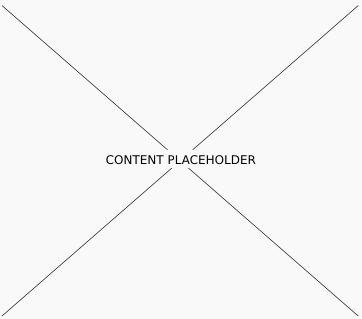
\includegraphics[width=0.9\linewidth]{figures/placeholder.png}
  \caption{Cute picture of robot tying knot}
  \label{fig:frontfig}
\end{figure}

In this paper, we present a solution to the demonstration selection problem that can account for the generalizability of demonstrations and the sequential nature of our applications.
Given a set of demonstrations and a method for generalizing them, we construct a discrete action abstract MDP.
Each action in this MDP is associated with a demonstration and our transition function is defined as applying trajectory transfer to generalize that demonstration.

This construction allows us to learn a Q function from example sequences of state-demonstration pairs.
This is accomplished through a max margin optimization problem whose solution captures the optimality of the examples and the temporal constraints imposed by the sequential nature of our tasks.
Our objective is a linear combination of features which are completely task agnostic and can be applied to any problem where trajectory transfer applies. 
We investigate the utility of this approach in a challenging knot-tieing scenario and show that the greedy application of our learned policy outperforms the nearest-neighbor baseline on a challenging distribution of problems. 
We leverage the fact that we learn a Q function representation of our policy (as opposed to a direct mapping from features to actions) to use a beam search to get near perfect performance in this task.
Finally, we present a method for bootstraping, though a process we call Leave-One-Out-Labelling, that enables us to do Max Margin Q-Learning with no additional human supervision beyond the initial demonstrations.

The rest of this paper is organized as follows: \dhm{fill this in later once we've drafted everything else}




\section{Technical Background}

\subsection{Trajectory Transfer through Non-Rigid Registration}
Non-rigid registration computes a function $f$ that minimizes error between landmark points, subject to a regularization term.
A commonly-used, effective method for registering spatial data is the Thin Plate Spline (TPS) regularizer \dhm{Cite Wahba, other stuff}.
Given a set of correspondence points $(x_i, y_i)$, we minimize the following objective:
$$\min_f \sum_i ||x_i - y_i||^2 + C\int dx ||D^2(f)||^2_{Frob}$$,
%%PA: move "," before the $$ for proper typesetting
where $C$ is a hyper-parameter that trades off between correspondance error and increased curvature.
This problem has a finite dimensional solution in terms of basis functions around the correspondence points.
The reader is referred to \dhm{cite survey on TPS} for more details.

Schulman et al. %%PA: citation missing
leverage TPS to perform trajectory transfer. 
Using a point cloud representation of both scenes, they use the TPS-RPM algorithm to jointy find point correspondances and a registration between them \dhm{Cite CHui}.
TPS-RPM alternates between (1) estimating correspondences between the point clouds of two scenes and (2) fitting the optimal TPS transformation based on these estimated scene correspondences. 
The result of this procedure is used to warp the path traced by the end effector of the robot in the demonstration.
Finally, this warped trajectory is used as a goal for trajectory following in order to find a similar trajectory that satisfies joint limits and collision constraints.
The result trajectory is executed, with the hope that the registration will account for changes in the environment but maintain the important aspects of the manipulation.

%%PA: i'd phrase this a bit differently; rather than considering each demonstration a policy; I'd say something about having an approach to generalize demonstrations to new situations;  hence a single demonstration can be seen as inducing a policy

%%PA: there is a lot of "Schulman et al" here; would be nice to just say that at the beginning of a paragraph stating Schulman et al present the following approach to ... :     and then describe everything in that paragraph;  
As a result, we can consider each demonstration as a policy that is parameterized by the environment around the robot.
Given a demonstration state, demonstration trajectory, and current state, the induced policy will produce a new trajectory to apply to the current state.
This approach has been effective in generalizing deformable object manipulations to new scenarios and has been explored for knot-tying and automated suturing.
Schulman et al. extend this method to make use of multiple demonstrations by computing the registration cost to several candidate demonstrations and selecting the demonstration with the lowest registration cost.
In this paper, we leverage trajectory transfer to generalize individual demonstrations, but describe a novel method for selecting from multiple demonstrations.
%%PA: some motivation in preceding sentence would be good; currently that sentence makes it sound as a really minor increment ... (which it isn't!)

\subsection{Structured Max Margin}
One way to incorporate expert demonstrations into learning in through the use of max-margin learning.
%%PA: in -> is
%%PA: overall this paragraph feels a bit wordy and not exactly paper-writing style "would like to" etc; how about cutting it straight to the point, and lead off with "Max-margin approaches ... " and say what they do in one sentence, and present the optimization problem, and describe what it encodes.
In this setting, we are given a set of labelled examples, \labelset{} (in our case pairings of states and expert demonstrations), and we would 
like to learn a function so that the labelled examples are all ranked highly.
To build a structured margin, we assume a similarity metric on labels, $m$,  so that we can leverage 
similarities and structure inherent to the problem.
The max-margin framework formalizes these desires through the following optimization problem:
\begin{equation}
\begin{aligned}
& \underset{w, \xi}{\text{minimize}}  & & ||w||^2 + C\sum \xi_i\\
& \text{subject to} & &w^\top \phi(\statevar{}_i, \actionvar{}_i) \geq w^\top \phi(\statevar{}_i, \actionvar{}') + m(\statevar{}_i, \actionvar{}_i, \actionvar{}') - \xi_i 
\\&&&\hspace{2.5cm}\forall (\statevar{}_i, \actionvar{}_i) \in \labelset{}, \forall \actionvar{}' \in \actionset{}\setminus \actionvar{}_i
\end{aligned}
\end{equation}


This approach has proven useful in many different scenarios where there is structure to an estimation or learning problem.
A notable, and related, example is that of Inverse Reinforcement Learning, where max-margin constrain reward functions that one might learn so that an expert's policy is optimal.
Maximum Margin Planning is one such application\dhm{CITE}. 
In it, the authors use maximum margin constraints for an MDP with known dynamics, but an unknown cost to place constraints on admissable cost functions.

%%PA: could subsection below be called Markov Decision Processes instead?
%%PA: also, do we really need to introduce the horizon?  It's good to minimize mental notational overhead; I think we can just say there are sink states where the process terminates which have a value of 0 ?  It'd be good to mention that to encode, let's say, tying a knot in a minimal number of segments, we could associate a reward of -1 with every segment execution.
%%PA: do we need the linear program here?  or can we just say that at the solution the Bellman equation is satisfied (and we already have the Bellman equations earlier on); followed by introducing linear function approximation and saying that when using function approximation one goes after weights that make the Bellman equations approximately satisfied; this would cut down the number of equations to one in the section below

\subsection{Q Function Approximation}
Markov Decision Processes are the formalization of choice for most stochastic sequential decision making problems.
They provide a way to account for stochasticity and there is a large array of techniques that can be used to solve them.
Formally, an undiscounted, finite-horizon, MDP, M, is represented as tuple $\langle\stateset,\actionset,T,R, H\rangle$~\cite{puterman1994}.
$\stateset{}$ is a set of states, that represent different configurations of our world.
$\actionset{}$ is a set of action we can take.
$T:\stateset{} \times \actionset{} \rightarrow \Delta_{\stateset{}}$ is a function that maps a state and action to a probability distribution over next states.
$R:\stateset{}\times \actionset{} \times \stateset{} \rightarrow \mathbb{R}$ is a function that specifies the reward our agent receives as a function of state, action, and next state.
$H$ is a horizon which determines the number of actions we will take in the MDP.
A solution to an MDP is a mapping from each state and horizon to an action.

The solution to an MDP is found by finding a value function, $V^*$, that satisfies the Bellman equations:
$${\footnotesize V(s, h) = \left\{ \begin{array}{cl} \underset{a}{\max}\ \underset{s'}{\sum} T(s, a, s')[R(s, a, s') + V(s', h-1)] & h >0 \\ 0 & h = 0\end{array}\right.}$$
It is sometimes easier to work with the right hand side of this equation, which we call a $Q$-function. Thus, $V^*(s, h) = \underset{a}{\max}Q^*(s, h, a)$.
There are many approaches to finding such a value function, but they require storing a vector that is $O(|\stateset{}|)$, which can be prohibitive in many applications. 


When faced with large state spaces, a common approach is to resort to value (or Q) function approximation~\cite{schweitzer1985generalized}. 
Given a set of basis functions $\phi: \stateset{}\times \actionset{} \rightarrow \mathbb{R}$ we can formulate an approximate linear program:
\begin{equation}
{\footnotesize
\begin{aligned}
\underset{w, \nu}{\min}\ \    &-w_0 + -\sum_{i, h} w^\top \phi(s_i, a_i, h) + C\sum \nu_i\\
\text{s.t.}\ \   &w^\top \phi(\statevar{}_i, \actionvar{}_i, h) \leq \\ &\ \ \ \ \ \ \underset{s'}{\sum}[R(s_i, a_i, s') + T(s_i, a_i, s')\underset{a'}{\max}\ w^\top \phi(\statevar{}'_i, \actionvar{}', h-1)] -  \nu_i \\
&w^\top \phi(\statevar{}_i, \actionvar{}_i, h) \leq 0
\end{aligned}}
\end{equation}
The solution to this optimization is a lower bound on the Q function of the MDP and have many fewer variables than the exact value function computation~\cite{puterman1994}.
However, we will still frequently have too many constraints in order to solve this optimization exactly.
Thus, many approximate linear programming techniques will further approximate by subsampling constraints.
While the result may no longer be an underestimator, contraints samples techniques have been quite successful in solving many large MDP problems.




\section{Related Work}
Related work for our contribution stems from three areas of research: deformable object manipulation (in particular knot-tieing), max margin policy learning, and \dhm{BLAH}
\subsection{Deformable Object Manipulation}
Our approach can be applied towards a variety of tasks in robotics,
including the manipulation of deformable objects.
In particular, we demonstrate the effectiveness of our approach for
knot tying, a commonly studied manipulation task in robotics.
Previous approaches to knot tying usually depend on rope-specific knowledge
and assumptions.
For instance, in knot planning from observation (KPO), knot theory is used
to recognize rope configurations and define movement primitives in visual
observations of humans tying knots \cite{Morita_ICRA2003, Takamatsu_TransRob2006}.
Existing motion planning approaches for knot tying use topological
representations of rope states (i.e. sequences of rope crossings and their
properties) and define a model for transitioning between topological states
\cite{Saha_ExpRobotics2008, Wakamatsu_IJRR2006}.
Robust open loop execution of knot tying has also been explored \cite{Bell_PhD2010}.

Recently, Schulman et al. used trajectory transfer to enable learning
from human-guided demonstrations of knot tying \cite{Schulmanetal_ISRR2013}.
For a given rope configuration, trajectory transfer is applied to the nearest
demonstration, and the resulting trajectory is executed.
The distance metric used is the thin plate spline (TPS) registration
cost between the rope configurations in the new scene and demonstration.
However, certain demonstrations may be less robust than others: for example,
a demonstration trajectory may involve a grasp that is unnecessarily near
the edge of a rope.
Our approach uses WillSmith to learn a policy that more robustly selects a
demonstration to apply, instead of always selecting the nearest demonstration.
\subsection{Max Margin Policy Learning}

\subsection{Inverse Optimal Control}
\et{I'm not really sure this is a subsection we want, just putting this here for
  now so the next sentence has a home.}  \citet{Dvijotham_ICML2010} also attempt
to directly learn a value function or Q-function for a MDP given sample
transitions generated by an optimal control policy. However, they assume either
a discrete state space or a linear dynamics model. In contrast, our method makes
no assumptions about the size of the state space or the dynamics model, instead
relying on segments of expert demonstrations as a means of navigating the state
space efficiently. \et{Someone who actually understands robotics should probably
  check this statement.}


\section{Problem Description and Formulation}
\label{sec:formulation}
%% Variables used across report
\newcommand{\actionset}{\ensuremath{\mathcal{A}}}
\newcommand{\actionsetsize}{\ensuremath{|\mathcal{A}|}}
\newcommand{\actionvar}{\ensuremath{a}}
\newcommand{\actionsub}[1]{\ensuremath{a_{#1}}}
\newcommand{\actionsubsup}[2]{\ensuremath{a_{#1}^{#2}}}

\newcommand{\demoset}{\ensuremath{\mathcal{D}}}
\newcommand{\demovar}{\ensuremath{d}}
\newcommand{\demosub}[1]{\ensuremath{d_{#1}}}
\newcommand{\demosubsup}[2]{\ensuremath{d_{#1}^{#2}}}

\newcommand{\trajset}{\ensuremath{\mathcal{T}}}

\newcommand{\labelset}{\ensuremath{\mathcal{L}}}
\newcommand{\labelsetsize}{\ensuremath{|\mathcal{L}|}}
\newcommand{\labelvar}{\ensuremath{\ell}}
\newcommand{\labelsub}[1]{\ensuremath{l_{#1}}}
\newcommand{\nsub}[1]{\ensuremath{n_{#1}}}
\newcommand{\sapairsub}[1]{\ensuremath{(s_{#1}, a_{#1})}}

\newcommand{\stateset}{\ensuremath{\mathcal{S}}}
\newcommand{\statevar}{\ensuremath{s}}
\newcommand{\statesub}[1]{\ensuremath{s_{#1}}}
\newcommand{\statesubsup}[2]{\ensuremath{s_{#1}^{#2}}}
\newcommand{\nextstatevar}{\ensuremath{s'}}
\newcommand{\transitionfn}{\ensuremath{T}}
\newcommand{\rewardfn}[1]{\ensuremath{R}}
\newcommand{\goalset}{\ensuremath{\mathcal{G}}}

\newcommand{\policyset}{\ensuremath{{\Pi}}}
\newcommand{\policyvar}{\ensuremath{\pi}}
\newcommand{\policysub}[2]{\ensuremath{\pi_{#1}(#2)}}

\newcommand{\regcost}{\ensuremath{r}}
\newcommand{\indexvar}{\ensuremath{i}}

\newcommand{\landmarkset}{\ensuremath{\mathcal{K}}}

\newcommand{\marginvar}{\ensuremath{m}}
\newcommand{\approxq}{\ensuremath{\tilde{Q}}}
\newcommand{\weights}{\ensuremath{w}}
\newcommand{\weightszero}{\ensuremath{w_0}}
\newcommand{\weightst}{\ensuremath{w^\intercal}}
\newcommand{\featurefn}{\ensuremath{\phi}}
\newcommand{\features}[2]{\ensuremath{\phi({#1}, {#2})}}
\newcommand{\marginslackc}{\ensuremath{C}}
\newcommand{\marginslacksubsup}[2]{\ensuremath{\xi_{#1}^{#2}}}
\newcommand{\bellmanslackc}{\ensuremath{D}}
\newcommand{\bellmanslacksubsup}[2]{\ensuremath{\nu_{#1}^{#2}}}
\newcommand{\bellmanc}{\ensuremath{F}}


In this section, we will formulate our approach to doing {\sc mmpl}, and
specify our assumptions regarding the problems it is applied to.

\subsection{Demonstration Set}

The required inputs of our pipeline are a set \demoset{}
of expert demonstrations and a set \labelset{} of labeled sequences of
task executions (Section~\ref{subsec:labeledex}).
Each \demovar{} $\in$ \demoset{} corresponds to a complete expert-guided
demonstration of the given robotic task or a movement primitive of a complete
demonstration --- our {\sc mmpl} formulation assumes the latter,
since it is often necessary for complex, multi-step tasks.
In our application of knot tying, we split each expert demonstration of
tying a knot into three or four movement primitives. The movement primitives
also include demonstration segments that attempt to
recover from failure states \cite{Schulmanetal_ISRR2013}.
Ideally, the segments in \demoset{} contain at least several demonstrations
of each movement primitive in the task.

A demonstration \demovar{} is composed of (\demosub{pc}, \demosub{traj}),
where \demosub{pc} is a point cloud representation of the underlying
starting state of the demonstration, and \demosub{traj} stores
the trajectory executed by the expert in that demonstration. The trajectory
space \trajset{} spans the set of all possible trajectories.


\subsection{Markov Decision Process Formulation}
Selecting from multiple demonstrations can be framed as a Markov Decision
Process (MDP), which enables us to apply Q-function approximation to derive a
policy.

In order to make planning in this space tractable, we use the set of
demonstrations \demoset{} to define a set of abstract actions \actionset{}. Each
action $\actionvar \in \actionset$ denotes the choice to use a corresponding
policy $\pi_d$, where we apply $\pi_d$ to some state $s$ by transferring
$d_{traj}$ to $s$ via TPS warping, then executing the resulting trajectory.

Since each action $\actionvar \in \actionset$ has a corresponding demo $\demovar
\in \demoset$, from here onward we refer to actions and demos
interchangeably. Additionally, $\policysub{d}{\statevar} =
\policysub{a}{\statevar}$ is most precisely defined as the trajectory that is
found via trajectory transfer from $\demovar$ to $\statevar$. However, since our
transition model is deterministic, applying this trajectory to $\statevar$ will
always produce the same successor $s'$. Thus, for ease of notation we will use
$\pi_{d}$ as the successor function for transferring $d_{traj}$ to a state $s$,
and say that $\policysub{d}{\statevar} = s'$.

Thus, the MDP for an \mmql{} problem is defined as
$\langle\stateset,\goalset,\actionset,T,R,H\rangle$, where

\begin{equation}
\begin{aligned}
\stateset{} &=  \text{all underlying states of the task} \\
\goalset{} &=  \text{all goal states of the task} \\
\actionset{} &= \{\policysub{\demovar{}}{\statevar{}}\ \mid \text{ } \demovar{} \in \demoset{}\} \\
\transitionfn{}(\statevar{}, \actionvar{}, \nextstatevar{}) &=
    \begin{cases}
    1[\policysub{\actionvar{}}{\statevar{}} = \nextstatevar{}] &\text{ if } \statevar{} \not \in \goalset{} \\
    1[\statevar{} = \statevar{}'] &\text{ if } \statevar{} \in \goalset{}
    \end{cases}\\
\rewardfn{}(\statevar{}) &= -1 {[ \statevar{} \not \in \goalset{} ]}. \\
H &= \text{finite horizon}
\end{aligned}
\end{equation}

In the above specification, \goalset{} denotes the goal set and contains all
states that satisfy the predefined goal. For example, in the knot-tying example,
\goalset{} denotes the set of tied knots.  Our MDP's reward function is then
simply $-1$ for all non-goal states and $0$ for goal states.

\subsection{Labeled Examples}
\label{subsec:labeledex}

As mentioned, one of the required inputs to our pipeline is a set \labelset{}
of labeled sequences of task executions. Each \labelsub{j} $\in$ \labelset{}
corresponds to a labeled sequence of
task executions of length \nsub{j}: \labelsub{j} = [\sapairsub{1},
\sapairsub{2}, \ldots, \sapairsub{\nsub{j}}]. Each labeled sequence corresponds
to a single complete task execution, ordered in the sequence of states and
actions taken. More formally, it is required that for each trajectory
\labelsub{j} $\in$ \labelset{}, for $1 \leq i \leq$ \nsub{j},
\begin{align*}
\transitionfn(\statesubsup{i}{(j)}, \actionsubsup{i}{(j)}) &= \statesubsup{i+1}{(j)} \text{ for } i < \nsub{j} \\
\text{and } T(\statesubsup{\nsub{j}}{(j)}, \actionsubsup{\nsub{j}}{(j)}) &\in \goalset{}
\end{align*}

\subsection{Max-Margin Q-Learning Formulation}
Our goal is to use the labeled sequences \labelset{} in order to learn an
approximate Q-function that determines, for a given state, which actions
rank higher than others.
Recall that actions in \actionset{} have a one-to-one correspondence with the
expert-guided demonstrations in \demoset{}, and are defined by executing the
transferred trajectory from the corresponding demonstration to the given state.

We approximate the Q-function for a given state \statevar{} and action
\actionvar{} as a linear combination of features \features{\statevar{}}{\actionvar{}}
(Section~\ref{sec:features}):
\begin{equation}
\approxq(\statevar{}, \actionvar{}) = \weightst{} \features{\statevar{}}{\actionvar{}}
\end{equation}

To calculate the weights, we construct an optimization problem within the
max-margin framework that incorporates max-margin constraints with a structured
margin, as well as Bellman constraints for Q-learning. The weights of \approxq{}
are then the solution of this optimization problem, which is as follows:
\begin{align}
& \underset{w, \xi, \nu}{\text{min}}  & & ||\weights{}||^2 + \marginslackc{} \sum_{j=1}^{\labelsetsize{}} \sum_{i=1}^{\nsub{j}} \marginslacksubsup{i}{(j)}
                                                      + \bellmanslackc{} \sum_{j=1}^{\labelsetsize{}} \bellmanslacksup{(j)} \notag \\
&    & & - \frac{\bellmanc{}}{\labelsatotal{}} \weightszero{} - \frac{\bellmanc{}}{\labelsatotal{}} \sum_{j=1}^{\labelsetsize{}} \sum_{i=1}^{\nsub{j}} \weightst{}\features{\statesubsup{i}{(j)}}{\actionsubsup{i}{(j)}}\\
& \text{s.t.} & &\weightst{} \features{\statesubsup{i}{(j)}}{\actionsubsup{i}{(j)}} \geq \weightst{} \phi(\statesubsup{i}{(j)}, \actionvar{}') + \marginvar{}(\statesubsup{i}{(j)}, \actionsub{i}, \actionvar{}') - \marginslacksubsup{i}{(j)} \notag\\
    &&&\hspace{1.9cm}\forall j = 1, \ldots, \labelsetsize{}; \text{ } \forall i = 1, \ldots, \nsub{j}; \notag\\
    &&&\hspace{1.9cm}\forall \actionvar{}' \in \actionset{}\setminus \actionvar{}_i  \label{eq:margin_constr}\\
&    & & \marginslacksubsup{i}{(j)} \geq 0 \hspace{0.7cm} \forall j = 1, \ldots, \labelsetsize{}; \text{ } \forall i = 1, \ldots, \nsub{j} \label{eq:margin_slacks}\\
&    & & \weightst{}\features{\statesubsup{i}{(j)}}{\actionsubsup{i}{(j)}} \leq \rewardfn{}(\statesubsup{i}{(j)}) + \weightst{}\features{\statesubsup{i+1}{(j)}}{\actionsubsup{i+1}{(j)}} + \bellmanslacksup{(j)} \notag \\
    &&&\hspace{1.9cm} \forall j = 1, \ldots, \labelsetsize{}; \text{ } \forall i = 1, \ldots, \nsub{j} - 2 \label{eq:bellman_constr}\\
&    & & \weightst{}\features{\statesubsup{\nsub{j}-1}{(j)}}{\actionsubsup{\nsub{j}-1}{(j)}} + \weightszero \leq \rewardfn{}(\statesubsup{\nsub{j}-1}{(j)}) + \bellmanslacksup{(j)} \notag \\
    &&&\hspace{1.9cm} \forall j = 1, \ldots, \labelsetsize{} \label{eq:bellman_goal_constr}\\
&    & & \bellmanslacksup{(j)} \geq 0 \hspace{0.7cm} \forall j = 1, \ldots, \labelsetsize{} \label{eq:bellman_slack}
\end{align}

where \labelsatotal{} is equal to the total number of
(\statevar{}, \actionvar{}) pairs in \labelset{}, so \labelsatotal{} = 
$\sum_{j=1}^{\labelsetsize{}} \sum_{i=1}^{\nsub{j}} 1$.

In the optimization problem, the constraints in Equation~\ref{eq:margin_constr}
enforce the max-margin requirements that the
labeled example's action \actionsubsup{i}{(j)} for state \statesubsup{i}{(j)}
has a higher (approximate) Q-value than the other actions for that
state. The slack variables \marginslacksubsup{i}{(j)} relax these constraints;
the degree of relaxation is controlled by the regularization parameter \marginslackc{}.
We build a structured margin, that allows actions similar to the
action of the labeled example to have a higher approximate Q-value.
We structure our margin with a similarity metric
\marginvar{}(\statesubsup{i}{(j)}, \actionsub{i}, \actionvar{}') that computes
the difference between the trajectories of the actions after being warped onto
the state \statesubsup{i}{(j)}. More precisely, we first apply trajectory
transfer on both actions \actionsub{i} and \actionvar{}' to transfer
each trajectory to the state \statesubsup{i}{(j)}. Then, we use dynamic
time warping of the trajectories for robust comparison of trajectories that
vary in time and speed. \sh{Add citation here for DTW}

The Bellman constraints in Equation~\ref{eq:bellman_constr} and~\ref{eq:bellman_goal_constr}
are key for learning a valid Q-function approximation \approxq. These constraints specify that
the values of the states in the labeled example task executions increase as they
approach the goal. In the objective, we effectively maximize the sum of the
approximate Q-values of the non-goal state-action pairs in the labeled examples,
thus driving the Bellman constraints to equality. By enforcing the value of goal states
to be zero, we arrive at the constraints in Equation~\ref{eq:bellman_goal_constr} for
states immediately prior to the goal in the labeled sequences.
The \weightszero{} term allows for the \approxq{} to be affine; it exists on
both sides of the inequality of Equation~\ref{eq:bellman_constr} and thus cancels out.
We can also ignore \weightszero{} when using \approxq{} to define a policy. The slack variables
\bellmanslacksup{(j)} relax these constraints, with \bellmanslackc{} controlling
the degree of relaxation.
\rewardfn{}(\statevar{}) is as defined in Equation~\ref{eq:mdp},
-1 for non-goal states and 0 for goal states.

\subsection{Leave-One-Out Labeling}
\label{subsec:lool}
One major limitation of the formulation we have outlined is its dependence on
the set of labeled sequences \labelset{}. We now propose an alternative method
of bootstrapping the set of expert demonstrations \demoset{} to generate an
unsupervised set of labeled sequences, $\labelset{}_u$, and we refer to this
method as leave-one-out labeling.

For each demonstration $\demovar{} \in \demoset{}$, we generate a corresponding
$\labelvar \in \labelset_u$ as follows. For every other demonstration
$\demovar{}' \neq \demovar{} \in \demoset{}$, we simply compute the TPS
registration cost between $\policysub{\demovar{}'}{d_{pc}}$ and
$\policysub{\demovar{}}{\demovar{}_{pc}}$. We choose the $\demovar{}^*$ with the
lowest registration cost, and add $(\demovar{}_{pc}, \demovar{}^*_{traj})$ to
$\labelset{}_u$ as an expert demonstration. Intuitively, this procedure looks to
discover the expert demonstration $d'$ that, when applied to the start state of
$d$, most closely mimics the optimal choice provided by the expert.

This method of labeling requires slight modifications to our max-margin
formulation. Since the expert's trajectory is assumed to be optimal for its
corresponding state, we exclude each expert demonstration from the max margin
constraints its corresponding unsupervisedexample generates. Additionally, note
that this unsupervised method of generating labeled sequences does not include a
temporal component. Thus, when forming the optimization problem with
$\labelset{}_u$, we must omit Bellman constraints. \et{If time/space permits
  this is where I'd talk about the second round of bootstrapping.}


\section{Results}
\label{sec:results}
% Variables used across report
\newcommand{\actionset}{\ensuremath{\mathcal{A}}}
\newcommand{\actionsetsize}{\ensuremath{|\mathcal{A}|}}
\newcommand{\actionvar}{\ensuremath{a}}
\newcommand{\actionsub}[1]{\ensuremath{a_{#1}}}
\newcommand{\actionsubsup}[2]{\ensuremath{a_{#1}^{#2}}}

\newcommand{\demoset}{\ensuremath{\mathcal{D}}}
\newcommand{\demovar}{\ensuremath{d}}
\newcommand{\demosub}[1]{\ensuremath{d_{#1}}}
\newcommand{\demosubsup}[2]{\ensuremath{d_{#1}^{#2}}}

\newcommand{\trajset}{\ensuremath{\mathcal{T}}}

\newcommand{\labelset}{\ensuremath{\mathcal{L}}}
\newcommand{\labelsetsize}{\ensuremath{|\mathcal{L}|}}
\newcommand{\labelvar}{\ensuremath{\ell}}
\newcommand{\labelsub}[1]{\ensuremath{l_{#1}}}
\newcommand{\nsub}[1]{\ensuremath{n_{#1}}}
\newcommand{\sapairsub}[1]{\ensuremath{(s_{#1}, a_{#1})}}

\newcommand{\stateset}{\ensuremath{\mathcal{S}}}
\newcommand{\statevar}{\ensuremath{s}}
\newcommand{\statesub}[1]{\ensuremath{s_{#1}}}
\newcommand{\statesubsup}[2]{\ensuremath{s_{#1}^{#2}}}
\newcommand{\nextstatevar}{\ensuremath{s'}}
\newcommand{\transitionfn}{\ensuremath{T}}
\newcommand{\rewardfn}[1]{\ensuremath{R}}
\newcommand{\goalset}{\ensuremath{\mathcal{G}}}

\newcommand{\policyset}{\ensuremath{{\Pi}}}
\newcommand{\policyvar}{\ensuremath{\pi}}
\newcommand{\policysub}[2]{\ensuremath{\pi_{#1}(#2)}}

\newcommand{\regcost}{\ensuremath{r}}
\newcommand{\indexvar}{\ensuremath{i}}

\newcommand{\landmarkset}{\ensuremath{\mathcal{K}}}

\newcommand{\marginvar}{\ensuremath{m}}
\newcommand{\approxq}{\ensuremath{\tilde{Q}}}
\newcommand{\weights}{\ensuremath{w}}
\newcommand{\weightszero}{\ensuremath{w_0}}
\newcommand{\weightst}{\ensuremath{w^\intercal}}
\newcommand{\featurefn}{\ensuremath{\phi}}
\newcommand{\features}[2]{\ensuremath{\phi({#1}, {#2})}}
\newcommand{\marginslackc}{\ensuremath{C}}
\newcommand{\marginslacksubsup}[2]{\ensuremath{\xi_{#1}^{#2}}}
\newcommand{\bellmanslackc}{\ensuremath{D}}
\newcommand{\bellmanslacksubsup}[2]{\ensuremath{\nu_{#1}^{#2}}}
\newcommand{\bellmanc}{\ensuremath{F}}




\section{Conclusions and Future Work}
In summation, we present a method for improving the use of trajectory transfer in 
learning from demonstrations for deformable object manipulation. 
We formulate this problem as a sequential decision making
problem in the form of a discrete-action abstract MDP. We present a novel approach to 
learning from demonstrations for this MDP, which we call Max-Margin Q-Learning, that 
integrates behavior cloning and value function approximation. We provide
features for learning in this scenario that make no additional assumptions beyond
the assumptions required to apply trajectory transfer. We describe Leave-One-Out Labeling 
for bootstrapping demonstrations in this MDP from only the intial demonstrations in our
trajectory library.

We validate our approach on a simulated knot-tying task and contribute a benchmark
set of examples (both at the low-level trajectory level and in the abstract MDP) and 
problems. We show a significant improvement over a baseline method that uses
a registration cost from trajectory transfer to select actions. We show that our learning
method is very data efficient and achieves close to peak performance with few examples.

There are several next steps to take in furthering this line of work. The first is to
expand on Leave-One-Out Labeling to incorporate Bellman constraints and make lookahead 
feasible. We believe this can be done through an application of reinforcement learning.
We can use the automatically labeled examples to initialize a policy for our task and then
use exploration to determine Bellman constraints needed for optimization. This provides
a nice method to incorporate experience into an expert demonstration.


\section{Section}

Section text here. 

\subsection{Subsection Heading Here}
Subsection text here.

\subsubsection{Subsubsection Heading Here}
Subsubsection text here.


\section{RSS citations}

Please make sure to include \verb!natbib.sty! and to use the
\verb!plainnat.bst! bibliography style. \verb!natbib! provides additional
citation commands, most usefully \verb!\citet!. For example, rather than the
awkward construction 

{\small
\begin{verbatim}
\cite{kalman1960new} demonstrated...
\end{verbatim}
}

\noindent
rendered as ``\cite{kalman1960new} demonstrated...,''
or the
inconvenient 

{\small
\begin{verbatim}
Kalman \cite{kalman1960new} 
demonstrated...
\end{verbatim}
}

\noindent
rendered as 
``Kalman \cite{kalman1960new} demonstrated...'', 
one can
write 

{\small
\begin{verbatim}
\citet{kalman1960new} demonstrated... 
\end{verbatim}
}
\noindent
which renders as ``\citet{kalman1960new} demonstrated...'' and is 
both easy to write and much easier to read.
  
\subsection{RSS Hyperlinks}

This year, we would like to use the ability of PDF viewers to interpret
hyperlinks, specifically to allow each reference in the bibliography to be a
link to an online version of the reference. 
As an example, if you were to cite ``Passive Dynamic Walking''
\cite{McGeer01041990}, the entry in the bibtex would read:

{\small
\begin{verbatim}
@article{McGeer01041990,
  author = {McGeer, Tad}, 
  title = {\href{http://ijr.sagepub.com/content/9/2/62.abstract}{Passive Dynamic Walking}}, 
  volume = {9}, 
  number = {2}, 
  pages = {62-82}, 
  year = {1990}, 
  doi = {10.1177/027836499000900206}, 
  URL = {http://ijr.sagepub.com/content/9/2/62.abstract}, 
  eprint = {http://ijr.sagepub.com/content/9/2/62.full.pdf+html}, 
  journal = {The International Journal of Robotics Research}
}
\end{verbatim}
}
\noindent
and the entry in the compiled PDF would look like:

\def\tmplabel#1{[#1]}

\begin{enumerate}
\item[\tmplabel{1}] Tad McGeer. \href{http://ijr.sagepub.com/content/9/2/62.abstract}{Passive Dynamic
Walking}. {\em The International Journal of Robotics Research}, 9(2):62--82,
1990.
\end{enumerate}
%
where the title of the article is a link that takes you to the article on IJRR's website. 


Linking cited articles will not always be possible, especially for
older articles. There are also often several versions of papers
online: authors are free to decide what to use as the link destination
yet we strongly encourage to link to archival or publisher sites
(such as IEEE Xplore or Sage Journals).  We encourage all authors to use this feature to
the extent possible.

\section{Conclusion} 
\label{sec:conclusion}

The conclusion goes here.

\section*{Acknowledgments}

%% Use plainnat to work nicely with natbib. 

\bibliographystyle{plainnat}
\bibliography{references}

\end{document}


